\documentclass[
    reds, % Saisir le nom de l'institut rattaché
    ie, % Saisir le nom de l'orientation
    %confidential, % Décommentez si le travail est confidentiel
]{heig-tb}

\usepackage[nooldvoltagedirection,european,americaninductors]{circuitikz}
\usepackage{todonotes}

%% Custom packages
\usepackage{multirow}

\signature{signature/kjordil} %TODO modifier le fichier de la signature (doit être un pdf)

\makenomenclature
\makenoidxglossaries
\makeindex

\addbibresource{bibliography.bib}

\usepackage{etoolbox}
\renewcommand\nomgroup[1]{%
  \item[\bfseries
  \ifstrequal{#1}{A}{Constantes physiques}{%
  \ifstrequal{#1}{B}{Groupes}{%
  \ifstrequal{#1}{C}{Autres Symboles}{}}}%
]}

\newcommand{\nomunit}[1]{%
\renewcommand{\nomentryend}{\hspace*{\fill}#1}}

\nomenclature[A, 02]{\(c\)}{\href{https://physics.nist.gov/cgi-bin/cuu/Value?c}
{Vitesse de la lumière dans le vide}
\nomunit{\SI{299792458}{\meter\per\second}}}

\nomenclature[A, 03]{\(h\)}{\href{https://physics.nist.gov/cgi-bin/cuu/Value?h}
{Constante de Planck}
\nomunit{\SI[group-digits=false]{6.62607015e-34}{\joule\per\hertz}}}

\nomenclature[A, 01]{\(G\)}{\href{https://physics.nist.gov/cgi-bin/cuu/Value?bg}
{Constante de gravitation universelle}
\nomunit{\SI[group-digits=false]{6.67430e-11}{\meter\cubed\per\kilogram\per\second\squared}}}

\nomenclature[B, 03]{\(\mathbb{R}\)}{Nombres réels}
\nomenclature[B, 02]{\(\mathbb{C}\)}{Nombres complexes}
\nomenclature[B, 01]{\(\mathbb{H}\)}{Quaternions}

\nomenclature[C]{\(V\)}{Volume constant}
\nomenclature[C]{\(\rho\)}{Indice de frottement sec}

% \newacronym{gcd}{GCD}{Plus grand diviseur commun} exemple d'acronyme
\newacronym{tb}{TB}{Travail de bachelor}
\newacronym{heigvd}{HEIG-VD}{Haute Ecole d'Ingénierie et de Gestion du Canton de Vaud}

\newglossaryentry{heig}{ %l'id que tu vas appeler dans ton texte
    name=HEIG-VD, % Ce qui s'affiche dans le texte
    description={Haute École d'Ingénierie et de Gestion du canton de Vaud} % La description à la fin du document
} 
\newglossaryentry{iai}{ %l'id que tu vas appeler dans ton texte
    name=IAI, % Ce qui s'affiche dans le texte
    description={Institut d'Automatisation industrielle} % La description à la fin du document
} 
\newglossaryentry{crc}{ %l'id que tu vas appeler dans ton texte
    name=CRC, % Ce qui s'affiche dans le texte
    description={Contrôle de redondance cyclique} % La description à la fin du document
} 
\newglossaryentry{framework}{
    name={framework},
    description={Un framework en programmation informatique est un ensemble structuré de composants logiciels qui offre une architecture cohérente et des directives pour le développement d'applications, en fournissant des fonctionnalités prédéfinies et un cadre de travail pour les développeurs}
}

% Auteur du document (étudiant-e) en projet de Bachelor
\author{Kévin Jordil}

% Activer l'option pour l'accord du féminin dans le texte
\genre{male}

% Titre de votre travail de Bachelor
\title{Framework pour écosystème décentralisé sur I2C}

% Le sous titre est optionnel
\subtitle{Travail de Bachelor}

% Nom du professeur responsable
\teacher {Prof. Y. Chevallier (HEIG-VD)}

% Mettre à jour avec la date de rendu du travail
\date{\today}

% Numéro de TB
\thesis{7212}



\surroundwithmdframed{minted}

%% Début du document
\begin{document}
\selectlanguage{french}
\maketitle
\frontmatter
\clearemptydoublepage

%% Requis par les dispositions générales des travaux de Bachelor
\preamble
\authentification

%% Résumé / Version abbrégée
\begin{abstract}
    % Francais
Le projet vise le développement d'un \textit{framework} pour écosystème décentralisé sur I2C.
Dans ce contexte, le projet vise principalement à résoudre certains problèmes rencontrés au sein du club de robotique de la Haute Ecole d'Ingénierie et de Gestion du Canton de Vaud (HEIG-VD) lors du concours international de robotique amateur, Eurobot.
Il a également pour objectif de résoudre des problèmes dans des projets industriels menés au sein de l'institut Reconfigurable \& embedded Digital Systems (REDS) et de l'Institut d'Automatisation industrielle (IAI).
L'objectif est d'améliorer l'efficacité et la réutilisabilité des composants tout en réduisant les coûts de développement et en optimisant les performances.

Le projet offre également une opportunité de relever les défis techniques et logistiques liés à la gestion des dispositifs, en combinant des aspects logiciels et matériels essentiels.
Le processus comprend une phase d'analyse, suivi d'une implémentation et enfin des tests, permettant ainsi la mise en place du \textit{framework} pour écosystème décentralisé sur I2C.

Au terme de ce développement, il est désormais possible de détecter les périphériques compatibles avec l'écosystème sur le bus I2C en affichant toutes les données correspondantes.
De plus, il est maintenant possible de mettre à jour le micrologiciel des composants via le bus I2C.

\asterism

% English
The project aims at developing a framework for a decentralized ecosystem on I2C.
In this context, the main objective of the project is to address specific issues encountered within the Robotics Club of the Haute Ecole d’Ingénierie et de Gestion du Canton de Vaud (HEIG-VD) during the international amateur robotics competition, Eurobot.
Additionally, it aims to solve problems in industrial projects carried out within the Reconfigurable \& embedded Digital Systems (REDS) Institute and the Institut d'Automatisation industrielle (IAI).
The goal is to improve component efficiency and reusability while reducing development costs and optimizing performance.

It also offers an opportunity to tackle technical and logistical challenges related to device management, combining essential software and hardware aspects.
The process involves an analysis phase, followed by implementation and testing, ultimately leading to the establishment of the framework for the decentralized ecosystem on I2C.

After completing this development, it is now possible to detect devices compatible with the ecosystem on the I2C bus by displaying all corresponding data.
Furthermore, updating firmware for components through the I2C bus is now achievable.
\end{abstract}

%% Sommaire et tables
\clearemptydoublepage
{
    \tableofcontents
    \let\cleardoublepage\clearpage
    \listoffigures
    \let\cleardoublepage\clearpage
    \listoftables
    \let\cleardoublepage\clearpage
    \listoflistings
}

\printnomenclature
\clearemptydoublepage
\pagenumbering{arabic}

%% Contenu
\mainmatter
\chapter{Introduction}
Dans le domaine des systèmes embarqués, l'utilisation de modules indépendants à microcontrôleurs est souvent nécessaire pour répartir les tâches et renforcer la modularité et la robustesse des systèmes.
Cependant, la communication entre ces modules représente un défi majeur.
C'est là qu'intervient le bus I2C, un protocole de communication simple et efficace permettant de connecter plusieurs modules à un seul bus.

Malgré les avantages du bus I2C, il présente certaines limitations.
Par exemple, il ne dispose pas d'une couche de gestion d'adresse, ce qui rend la maintenance complexe lorsque plusieurs micrologiciels sont nécessaires pour faire fonctionner l'écosystème.
De plus, la gestion des mises à jour des modules et la gestion des erreurs de communication posent également des problèmes.

C'est dans ce contexte que ce projet vise à développer un framework innovant pour la gestion d'un écosystème décentralisé sur un bus I2C.
L'objectif principal est de créer une solution qui permette de gérer les adresses des modules, d'assurer les communications entre ces derniers, ainsi que de faciliter le déploiement automatique de nouveaux micrologiciels sur les modules et la gestion des mises à jour.

Pour atteindre ces objectifs, ce projet se déroulera en plusieurs étapes.
Tout d'abord, une sélection sera effectuée pour choisir un microcontrôleur compact disposant des périphériques courants et programmable en langage C/C++.
De préférence, ce microcontrôleur sera compatible avec le framework mbed et basé sur une architecture ARM, comme Cortex-M0+ ou Cortex-M4.

Ensuite, un bootloader sera développé ou utilisé, tel que u-boot, pour permettre le déploiement automatique des nouveaux micrologiciels sur les modules via le bus de communication.
Ce bootloader devra être compatible avec le framework mbed, et la gestion des versions firmware se fera à l'aide d'un hash.

À l'issue de ce travail, plusieurs tâches clés seront accomplies, notamment le développement d'un écosystème I2C pour les microcontrôleurs, la sélection d'un framework de développement adapté, le choix d'un microcontrôleur approprié, l'implémentation d'un système d'auto-adressage des éléments du bus, ainsi que la création d'un bootloader permettant la mise à jour automatique des micrologiciels embarqués.
De plus, une interface POSIX sera développée pour faciliter l'interaction avec les éléments du bus.
Un démonstrateur du système sera réalisé, mettant en évidence toutes les fonctionnalités mentionnées précédemment.
Le code source de ce projet sera livré sous GitHub, accompagné d'une documentation adéquate.

En résumé, ce projet vise à développer un framework novateur pour la gestion d'un écosystème décentralisé sur le bus I2C, en apportant des solutions aux problèmes de gestion d'adresses, de communication, de déploiement de micrologiciels et de maintenance.
L'objectif final est de faciliter la mise en place et la gestion de systèmes embarqués modulaires et robustes, tout en offrant une flexibilité et une fiabilité accrues.

\section{Contexte}
Le club de robotique de l'HEIG participe au concours international de robotique amateur, Eurobot.
Ce concours met en compétition des équipes de jeunes, qu'elles soient constituées d'étudiants ou de clubs indépendants.
Au fil des années, il est apparu que la gestion des capteurs présents sur les robots était un besoin essentiel.
En effet, chaque année, les robots doivent être adaptés aux nouvelles contraintes du concours.
Toutefois, de nombreux capteurs utilisés restent les mêmes d'une année à l'autre.
Par conséquent, il serait intéressant de pouvoir réutiliser facilement ces capteurs.
C'est dans ce contexte que ce projet a été proposé.

Sur le marché, les capteurs disponibles offrent des interfaces de communication qui diffèrent d'un capteur à l'autre.
L'objectif de ce projet est donc de créer un écosystème regroupant tous les capteurs sur un même bus de communication, facilitant ainsi leur intégration dans les robots.
De plus, il est nécessaire de mettre en place une gestion des mises à jour des capteurs via le protocole de communication utilisé.

En développant cet écosystème, cela vise à améliorer l'efficacité et la réutilisabilité des capteurs d'année en année, ce qui permettra de réduire les coûts de développement et d'optimiser les performances des robots.
La création d'un système de communication unifié et la mise en place d'une procédure de mise à jour simplifiée contribueront à rendre le processus de développement plus efficace et plus fluide.

Ce projet représente une occasion exceptionnelle de relever le défi technique et logistique de la gestion des capteurs dans le cadre d'une compétition robotique.
En effet, il combine à la fois des aspects logiciels et matériels essentiels.
Étant donné que l'espace disponible à l'intérieur d'un robot est limité, il est primordial de concevoir un système compact et efficace.
De plus, la gestion des capteurs doit être à la fois simple et performante afin de permettre son utilisation par les étudiants tout au long de leur cursus de bachelor.
\chapter{Cahier des charges}
Ce rapport a été réalisé dans le cadre d'un travail de bachelor à l'\gls{heig} en 2023.
Les objectifs définis dans le cahier des charges sont les suivants :

\begin{itemize}
    \item Un écosystème \gls{i2c} doit être développé pour les microcontrôleurs.
    \item Un \textit{\gls{framework}} de développement doit être choisi.
    \item Un microcontrôleur doit être sélectionné.
    \item Les éléments du bus doivent s'auto-adresser et être identifiés par un identifiant unique.
    \item Un chargeur de démarrage doit être mis en place pour permettre la mise à jour du micrologiciel embarqué.
    \item Une interface POSIX doit être développée pour interagir avec les éléments du bus.
    \item Un démonstrateur du système couvrant les points susmentionnés doit être réalisé.
    \item Le code doit être livré sur GitHub, accompagné d'une documentation adéquate.
\end{itemize}

Il existe également des objectifs qui peuvent être réalisés si le temps le permet :

\begin{itemize}
    \item Une carte électronique dédiée avec un capteur et/ou un afficheur doit être réalisée.
    \item La mise en place d'un CI/CD (Continuous Integration/Continuous Deployment).
\end{itemize}


\chapter{Analyse}
Dans ce chapitre, l'objectif est d'effectuer une analyse approfondie de chaque composant du système afin de déterminer leurs caractéristiques et spécifications respectives.
Cette analyse permettra ensuite de sélectionner les composants à utiliser pour la réalisation du système.

\section{Bus de communication}

Dans le cadre de ce projet, le bus de communication envisagé est l'\gls{i2c}.
Cependant, il est pertinent de comparer ce bus avec d'autres protocoles de communication pour déterminer le plus adapté.
Il existe une variété de bus de communication disponibles.
Pour ce projet, il est nécessaire de choisir un protocole simple et compact, en accord avec les exigences des systèmes embarqués.

Dans ce projet, le nombre maximal de périphériques n'est pas clairement défini.
Il est donc important de sélectionner un protocole offrant une capacité maximale en termes de nombre de périphériques, afin de ne pas être limité par cette contrainte à l'avenir.

La vitesse de transfert des données doit être suffisante pour permettre la transmission des informations des capteurs et des actionneurs.
Cependant, la vitesse de transfert des données n'est pas un critère critique pour ce projet.

Enfin, le nombre de fils de communication est un paramètre important à prendre en compte.
En effet, il est nécessaire de limiter au maximum le nombre de fils de communication afin de prévenir la complexité du câblage et de réduire l'encombrement.

Afin de faciliter cette comparaison, un tableau comparatif des différents bus de communication pertinents pour ce projet est présenté ci-dessous.

\begin{table}[H]
    \begin{center}
        \caption{Bus de communication \label{tab:buscommunication}}
        \begin{tabular}{c|c|c|c}
            Nom & \begin{tabular}[c]{@{}c@{}}Nombre maximal\\ de périphériques\end{tabular} & Vitesse standard & Fils de communication \\ \hline
            \gls{i2c} & 127                                                                       & 0.1 Mbit/s       & 2                     \\
            CAN & Non défini                                                                & 1 Mbit/s         & 2                     \\
            LIN & 16                                                                        & 0.02 Mbit/s      & 1                     \\
            SPI & Non défini                                                                & 10 Mbit/s        & 4
        \end{tabular}
    \end{center}
\end{table}

La vitesse spécifiée représente la vitesse standard du bus, mais dans certains cas, la vitesse peut être supérieure avec une autre configuration.

\subsection{LIN}

Le bus LIN est le bus de communication le plus lent et a un nombre réduit de périphériques par rapport aux autres.
Il est donc écarté.

\subsection{SPI}

Le bus SPI a une particularité, le nombre de fils de communication dépend du nombre de périphériques connectés.
En effet, il possède quatre signaux logiques : \texttt{SCLK} (Serial Clock) qui est l'horloge du bus, \texttt{MOSI} (Master Output Slave Input) qui est la ligne de données du maître vers l'esclave, \texttt{MISO} (Master Input Slave Output) qui est la ligne de données de l'esclave vers le maître et \texttt{SS} (Slave Select) qui est la ligne de sélection de l'esclave.
Le nombre de fils de communication est donc égal à trois plus le nombre de périphériques esclaves.
Ce bus ne convient pas à ce projet, car il n'est pas simple d'ajouter ou de retirer des périphériques.

\subsection{CAN}

Le bus CAN possède une vitesse intéressante par rapport aux autres bus de communication. Cependant, lorsqu'un composant fonctionne avec CAN, il utilise CANOpen. CANOpen est complexe à mettre en place. De plus la majorité des microcontrôleurs qui possède un contrôleur CAN doivent être connecté à un transceiver CAN qui est un autre composant. Ce bus n'est donc pas adapté à ce projet.

\subsection{I2C}

Le bus \gls{i2c} est vraiment adapté pour notre projet, car il ne présente pas de défauts majeurs par rapport à d'autres bus de communication.
De plus, la plupart des composants \gls{i2c} disponibles actuellement sur le marché prennent en charge le "fast mode" qui permet une vitesse de transfert allant jusqu'à 0.4 Mbit/s.

Une autre caractéristique intéressante de l'\gls{i2c} est son mode multimaître, qui peut être utile dans certaines situations.
En résumé, l'\gls{i2c} répond parfaitement à nos exigences pour ce projet, offrant une vitesse de transfert suffisante et la flexibilité nécessaire.

\section{Microcontrôleur}

Dans cette section, une analyse des microcontrôleurs disponibles sur le marché sera réalisée dans le but de déterminer celui qui convient le mieux à ce projet.
De plus, une évaluation des langages de programmation les plus couramment utilisés pour les microcontrôleurs sera effectuée.
Il sera également nécessaire de choisir le boîtier le plus approprié pour le microcontrôleur sélectionné.
Après ces analyses, d'autres critères devront être définis.
Par exemple, il est spécifié dans le cahier des charges que le microcontrôleur doit être équipé d'un ARM Cortex.
De plus, il est essentiel d'avoir les périphériques couramment utilisés tels que UART, SPI, \gls{i2c}, GPIO, ADC et PWM.
Ces critères devront être pris en compte lors du choix final du microcontrôleur.

\subsection{Fabricants}

Dans le domaine des microcontrôleurs, il existe plusieurs fabricants présents sur le marché.
Cependant, il est pertinent de se concentrer sur les fabricants qui détiennent une part de marché significative.
Cette approche garantit un accès à une documentation exhaustive ainsi qu'à un approvisionnement adéquat, en termes de disponibilité des composants.
Les données de \href{https://www.statista.com/statistics/1327509/top-mcu-suppliers-worldwide/}{Statista.com} fournissent un aperçu des parts de marché des fabricants de microcontrôleurs en 2021.
Voici un graphique présentant ces données.

\begin{figure}[H]
    \centering
    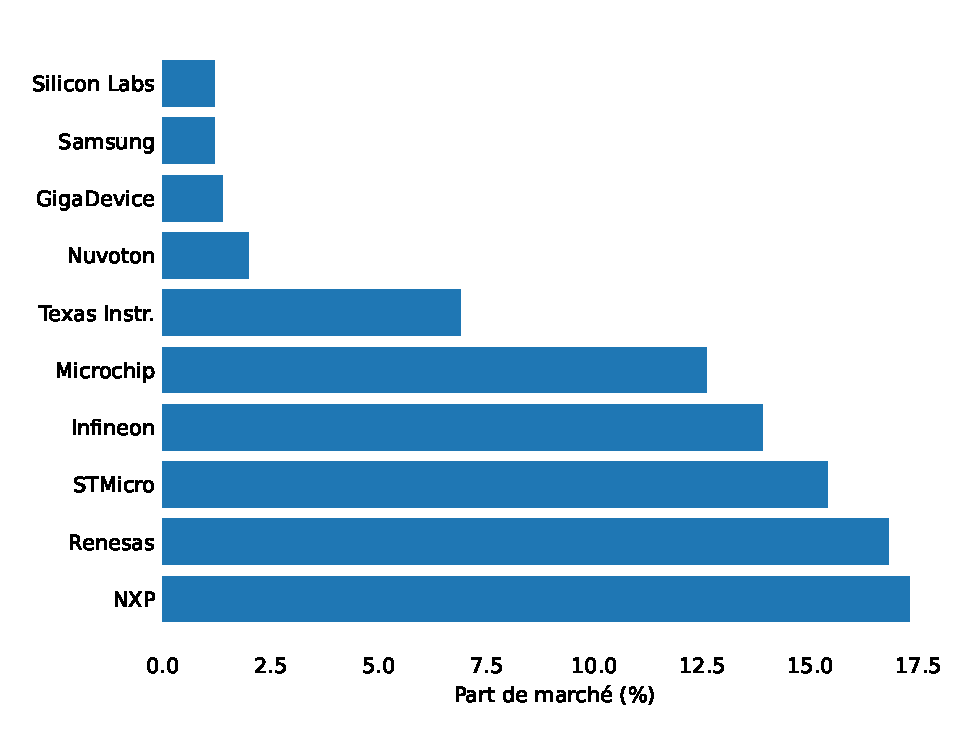
\includegraphics[width=12cm]{./assets/figures/topmcu.py.eps}
    \caption{Part de marché des fabricants de microcontrôleurs en 2021 }
    \label{fig:topmcu}
\end{figure}

L'analyse des données révèle que NXP, Renesas, STMicro, Infineon, Microchip et Texas Instruments sont les principaux fabricants de microcontrôleurs sur le marché en 2021.
Il est donc judicieux de considérer ces fabricants en priorité lors du processus de sélection du microcontrôleur.
Chacun des fabricants mentionnés ci-dessus propose des microcontrôleurs basés sur l'architecture ARM Cortex.

\subsection{Langages de programmation}

Différents langages de programmation sont utilisés pour programmer des microcontrôleurs, mais certains sont plus répandus que d'autres.
Le langage de programmation C est largement utilisé et constitue le choix prédominant lorsqu'il s'agit de trouver du code pour les microcontrôleurs.
Dans certains cas, l'assembleur est également utilisé, notamment pour des applications spécifiques.
Des projets utilisent également des langages tels que le C++, le Rust et le Python, bien que leur usage soit moins courant.
La première option courante consiste donc à utiliser le langage C.
Cependant, il est intéressant d'explorer les autres langages de programmation, en particulier le C++, afin de déterminer leur pertinence pour ce projet.

Le choix du langage de programmation dépendra des fonctionnalités et des possibilités offertes par le \textit{\gls{framework}} de développement sélectionné.

\subsection{Boitiers}

Les microcontrôleurs sont disponibles dans différentes tailles de boîtiers, chacun présentant ses avantages et ses inconvénients.
Dans le cadre de ce projet, il est essentiel de choisir un boîtier compact et facile à souder.
La taille réduite du boîtier est importante, car elle permet de minimiser l'empreinte du circuit imprimé, ce qui répond aux exigences de compacité des systèmes embarqués du projet.
La facilité de soudure est également un critère important, car elle permet de réduire les coûts de production et facilite la maintenance en permettant le remplacement facile des composants défectueux.
Ainsi, la sélection du boîtier approprié contribue à la performance et à la durabilité du projet.

Le boîtier BGA offre un excellent rapport taille/nombre de broches.
Cependant, il est difficile à souder sans équipement spécifique, il est donc exclu pour ce projet.

\begin{figure}[H]
    \centering
    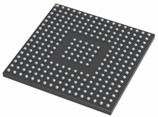
\includegraphics[scale=0.4]{./assets/figures/bga.jpg}
    \caption{\cite{bga} Boitier BGA}
\end{figure}

Le boîtier SO/SSOP est facile à souder, mais il présente une limitation en termes de nombre de broches et occupe beaucoup d'espace sur le circuit imprimé pour seulement deux rangées de broches.
Il est donc écarté.

\begin{figure}[H]
    \centering
    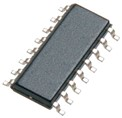
\includegraphics[scale=0.45]{./assets/figures/so_ssop.jpg}
    \caption{\cite{so_ssop} Boitier SO/SSOP}
\end{figure}

Le boîtier TQFP/LQFP est facile à souder, offre un plus grand nombre de broches que le boîtier SO/SSOP et occupe moins d'espace sur le circuit imprimé.
Il est donc intéressant pour ce projet.

\begin{figure}[H]
    \centering
    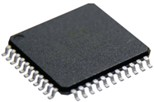
\includegraphics[scale=0.4]{./assets/figures/tqfp_lqfp.jpg}
    \caption{\cite{tqfp_lqfp} Boitier TQFP/LQFP}
\end{figure}

Enfin, le boîtier QFN est facile à souder pour quelqu'un d'expérimenté et offre un plus grand nombre de broches par rapport à sa taille.
Il occupe donc très peu d'espace sur le circuit imprimé.
Il est donc plus intéressant que le boîtier TQFP/LQFP, en tenant compte de la taille qui est un critère important pour ce projet.

\begin{figure}[H]
    \centering
    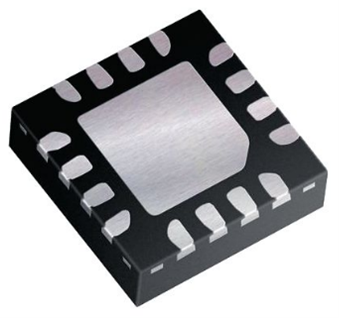
\includegraphics[scale=0.5]{./assets/figures/qfn.png}
    \caption{\cite{qfn} Boitier QFN}
\end{figure}

Ainsi, après évaluation, les boîtiers privilégiés pour ce projet sont le boîtier QFN en raison de sa compacité et de son nombre de broches plus élevé, et le boîtier TQFP/LQFP en raison de sa facilité de soudure et de son encombrement réduit par rapport au boîtier SO/SSOP.

\subsection{Choix}

Pour assurer la durabilité de ce projet, il est crucial de choisir un microcontrôleur largement utilisé, afin de pouvoir le remplacer par un modèle similaire de la même famille si celui-ci venait à être discontinué.

En Suisse, les principaux acteurs dans le domaine des sites marchands d'achat sont Digikey et Mouser.
Ces sites proposent généralement des produits similaires, avec des différences principalement liées à leur stock.
Cependant, Digikey offre un système de filtres qui permet de sélectionner les périphériques souhaités sur le microcontrôleur, ce qui est essentiel pour ce projet.
Les recherches seront donc effectuées sur Digikey.

Il convient d'appliquer les filtres suivants :

\begin{itemize}
    \item Processeur c\oe{}ur: ARM Cortex-M*
    \item En stock: Oui
    \item Connectivité: \gls{i2c}, UART, SPI
    \item Périphériques: PWM
    \item Boîtier: *QFN
    \item Boîtier fournisseur: Inférieur ou égal à (4x4)
\end{itemize}

Le choix d'un c\oe{}ur ARM Cortex-M assure une architecture ARM solide, idéale pour les systèmes embarqués.
En ce qui concerne la taille du boîtier, une dimension égale ou inférieure à 4x4mm garantit la compacité du microcontrôleur.

Cependant, il y a un critère qui ne peut pas être pris en compte lors de l'application des filtres, c'est la définition du nombre de bus \gls{i2c}.
En effet, il est nécessaire d'avoir deux bus de données \gls{i2c}.
Un qui fera partie de l'écosystème, et un autre qui permet, si nécessaire, de piloter un périphérique \gls{i2c}.
Il est donc essentiel de vérifier dans la fiche technique du microcontrôleur s'il dispose bien de deux bus \gls{i2c}.

Environ 80 résultats correspondent aux critères définis.
En analysant ces résultats, il est remarqué qu'il y a une présence significative de microcontrôleurs de la famille STM32.
Cette famille est étendue, ce qui en fait un choix privilégié.
Après avoir examiné les datasheets, deux microcontrôleurs répondent aux exigences du projet : le STM32G031G6U6 et le STM32G071GBU6.
La principale différence entre les deux réside dans la quantité de mémoire flash et de RAM.
Dans ce projet, l'objectif est d'utiliser un chargeur de démarrage et un micrologiciel.
Par conséquent, il est préférable de choisir le STM32G071GBU6 qui offre une plus grande capacité de mémoire flash et de RAM.
Cela évitera de rencontrer des problèmes de mémoire lorsque des fonctionnalités supplémentaires seront ajoutées ultérieurement dans le projet.

\section{Frameworks}

Pour assurer un fonctionnement simple, une maintenance aisée et une portabilité du code, l'utilisation d'un \textit{\gls{framework}} de développement est intéressante.
Celui-ci fait le lien entre un code plus abstrait et un code spécifique au microcontrôleur.
Il est important de pouvoir accéder aux fonctionnalités de bas niveau du microcontrôleur lorsque celles-ci ne sont pas réalisées de manière plus abstraite dans le \textit{\gls{framework}}.
Ainsi, il doit faciliter le développement de fonctionnalités spécifiques et disposer d'une documentation complète.
Il doit également être maintenu et utilisé par une communauté active, ce qui permet de trouver des solutions aux problèmes plus facilement.
De plus, le \textit{\gls{framework}} doit être compatible avec le microcontrôleur STM32 choisi.
Trois \textit{\gls{framework}s} potentiels répondent à ces critères, il s'agit de Mbed, Arduino et STM32Cube.
Il convient d'analyser et de comparer ces \textit{\gls{framework}s} pour déterminer lequel est le plus adapté à ce projet.

\subsection{Arduino}

Le \textit{\gls{framework}} Arduino est largement adopté par les amateurs d'électronique pour leurs projets personnels, mais il est moins couramment utilisé dans le milieu professionnel.
Bien qu'il permette une implémentation rapide des fonctionnalités, il peut manquer d'optimisation par rapport à une plateforme dédiée.
La communauté qui entoure Arduino est vaste, mais elle est principalement constituée d'amateurs.
La documentation disponible peut être moins claire, avec une prédominance de forums et de tutoriels orientés vers des projets personnels.
De plus, il n'existe pas de documentation officielle exhaustive pour chaque fonctionnalité avec des exemples spécifiques.

Une particularité d'Arduino réside dans le fait qu'il n'y a pas de licence open source unique pour ses bibliothèques.
Chaque bibliothèque peut avoir sa propre licence.
Cela peut poser des problèmes si une bibliothèque utilise la licence publique générale GNU (GPL).
Cette licence exige que le code source du projet soit disponible pour tous.
Cette situation peut être contraignante si l'on souhaite utiliser l'écosystème Arduino à des fins commerciales tout en maintenant le code source confidentiel.

\subsection{STM32Cube}

Le \textit{\gls{framework}} STM32Cube est développé par STMicroelectronics, le fabricant du microcontrôleur STM32, et il est intégré à l'IDE STM32CubeIDE.
Il offre une compatibilité optimale avec les microcontrôleurs STM32, permettant de tirer pleinement parti de leurs fonctionnalités.
Il offre une interface conviviale pour configurer les broches du microcontrôleur en fonction des fonctionnalités souhaitées.
Cependant, il peut être assez verbeux, ce qui signifie que l'utilisateur doit écrire son code dans des zones spécifiques et délimitées par des commentaires.
Cela peut rendre le code plus complexe à comprendre au premier abord, car il mélange les aspects bas niveau du microcontrôleur avec des fonctionnalités de haut niveau.

Lors de la recherche d'informations sur l'implémentation de fonctionnalités spécifiques, il peut être difficile de trouver une documentation officielle.
Cependant, les forums sont souvent une source précieuse d'informations, avec souvent des réponses fournies par des professionnels expérimentés.

\subsection{Mbed}

Mbed est un \textit{\gls{framework}} développé en collaboration par ARM et ses partenaires technologiques, spécialement conçus pour les microcontrôleurs ARM Cortex-M 32 bits.
Il offre une documentation officielle très complète, qui se classe souvent en tête des résultats de recherche lorsqu'il s'agit d'implémenter des fonctionnalités spécifiques.
Les forums Mbed sont également une ressource précieuse, avec une présence notable de professionnels expérimentés.

Ce qui est particulièrement avantageux avec Mbed, c'est sa simplicité pour mettre en place une communication complète.
La documentation officielle fournit de nombreux exemples pour la plupart des fonctionnalités, facilitant ainsi le développement.

En termes de licence, Mbed est open source, la plupart de ses composants étant sous licence BSD-3-Clause ou MIT.
Cela signifie que les utilisateurs ont la liberté d'utiliser, de modifier, de fusionner, de publier, de distribuer, de vendre et de sous-licencier le logiciel.
La seule condition est d'inclure la notice de licence et les droits d'auteur dans toutes les copies, ce qui offre une grande flexibilité pour les utilisations futures du projet, sans limiter la créativité.

\subsection{Choix}

Suite à l'analyse des trois \textit{\gls{framework}s}, Mbed est choisi comme le plus approprié pour ce projet.
Il répond de manière optimale aux critères définis.
Mbed dispose d'une documentation complète, abondamment illustrée d'exemples concrets.
Une communauté dynamique, principalement composée de professionnels expérimentés, anime les forums associés.
Le \textit{\gls{framework}} offre également un accès aux fonctionnalités de bas niveau du microcontrôleur, si besoin.
Par ailleurs, Mbed est un projet open source, accompagné d'une licence qui permet une grande flexibilité pour les futures utilisations du projet.

\section{Interface POSIX}

L'interface POSIX est employée pour interagir avec les éléments du bus, favorisant ainsi une communication efficace avec les divers composants \gls{i2c} et permettant d'exploiter pleinement les fonctionnalités développées dans ce projet.
Cette interface inclut la détection des périphériques connectés au bus, la récupération des informations détaillées sur ces périphériques et la mise à jour du micrologiciel.
Dans un souci de portabilité, l'interface sera implémentée en Python, un langage largement utilisé dans le domaine de l'embarqué, offrant une rapidité de développement des applications et une compatibilité avec de nombreux systèmes d'exploitation.

\subsection{Découverte des périphériques}

Dans Linux, il existe un outil appelé \texttt{i2cdetect} qui permet de détecter tous les périphériques connectés sur le bus \gls{i2c}.
Cet outil est issu du package \texttt{i2ctools}.
Cependant, il y a une subtilité à prendre en compte.
Par défaut, le programme effectue une lecture ou une écriture en fonction de l'adresse détectée.
Cette particularité est due au fait que certains microcontrôleurs, tels que les microcontrôleurs Atmel AT24RF08, se corrompent lorsqu'une écriture est effectuée.
À l'inverse, certains microcontrôleurs, notamment les microcontrôleurs d'horloge, ne répondent pas à une lecture, car ils sont en mode écriture seule.
Pour éviter ce problème, l'outil \texttt{i2cdetect} effectue des lectures ou des écritures en fonction de plages d'adresses connues correspondant aux composants problématiques.
Dans le cas de ce projet, il n'y a pas de composants posant problème, ce qui permet d'uniformiser le comportement en n'effectuant que des lectures.
Cela peut être réalisé en utilisant l'option \texttt{-r} de l'outil.

Dans le cadre de ce projet, il peut être intéressant de mettre en place une détection supplémentaire permettant de détecter uniquement les périphériques compatibles avec le projet.
À cet effet, un script Python a été développé.
Ce script permet de détecter les périphériques de l'écosystème en se basant sur une réponse prédéfinie.
Cela permet à l'utilisateur de distinguer rapidement et efficacement les périphériques compatibles avec le projet des autres périphériques présents sur le bus \gls{i2c}.

Lors de la détection des périphériques, plusieurs informations peuvent être affichées.
Cela comprend notamment l'adresse, la version du micrologiciel, le type de périphérique, le groupe de périphérique, le nom et l'identifiant unique.

\subsubsection{Adresse}

L'adresse \gls{i2c} d'un périphérique est intéressante à connaître, car elle permet d'utiliser le périphérique dans un autre contexte que celui de l'écosystème développé dans ce projet.

\subsubsection{Version du micrologiciel}

La version du micrologiciel présente sur le périphérique est également importante à connaître, car elle permet de comparer facilement les versions et de déterminer quels périphériques nécessitent une mise à jour éventuelle.

\subsubsection{Type de périphérique}

Le type de périphérique est utile pour faciliter la mise à jour du micrologiciel sur plusieurs périphériques simultanément.
Lorsqu'un code évolue pour un certain type de périphérique, il est avantageux de pouvoir mettre à jour tous les périphériques de ce type en même temps.

\subsubsection{Groupe de périphérique}

Le groupe de périphérique est un sous-filtre du type de périphérique, permettant de différencier des périphériques d'un même type.
Cela est particulièrement utile lorsque différents groupes de périphériques du même type présentent des fonctionnalités différentes, afin de ne mettre à jour que les périphériques concernés par les changements de firmware.

\subsubsection{Nom}

Le nom du périphérique est intéressant pour l'utilisateur. En effet, il permet de différencier les périphériques entre eux. Cela permet de faire un lien plus rapide entre l'affichage et le périphérique physique.

\subsubsection{Identifiant unique}

L'identifiant unique est un identifiant distinct attribué à chaque périphérique.
Il permet de différencier de manière unique les périphériques les uns des autres.
Cet identifiant est prédéfini par le fabricant et ne peut être modifié.
Grâce à ce champ, il est possible à tout moment de distinguer les périphériques entre eux de manière univoque.

\subsection{Mise à jour du micrologiciel}

La mise à jour du micrologiciel est une fonctionnalité clé de l'interface POSIX.
Elle permet de mettre à jour facilement et efficacement le micrologiciel des périphériques concernés, sans avoir besoin de connecter un câble spécifique pour la programmation de la carte.
En utilisant la commande de mise à jour appropriée, le programme est en mesure de téléverser le nouveau micrologiciel sur le périphérique cible.
Une fois la mise à jour terminée avec succès, le périphérique redémarre avec le nouveau micrologiciel.

La mise à jour du micrologiciel peut être réalisée en utilisant l'adresse \gls{i2c} du périphérique, le type de périphérique ou le groupe de périphériques.
Cette flexibilité permet de mettre à jour un ou plusieurs périphériques simultanément en exécutant une seule commande.

\section{Auto-adressage}

Sur un bus \gls{i2c}, chaque périphérique doit avoir une adresse unique.
Cependant, les périphériques utilisent la même méthode de génération, il est alors nécessaire de générer des adresses différentes tout en utilisant le même algorithme.
Il est donc important de trouver une méthode pour générer une adresse unique pour chaque périphérique.

\subsection{Méthode de génération}

La méthode de génération d'adresse repose sur l'utilisation de l'identifiant unique de chaque périphérique.
Grâce à cet identifiant, il est possible de générer une adresse différente pour chaque périphérique tout en utilisant le même algorithme.
Il est cependant essentiel de garantir l'unicité des adresses générées à partir de cet identifiant.

Dans un premier temps, il est nécessaire de définir une plage d'adresses dans laquelle les périphériques peuvent être adressés.
Pour ce projet, la plage d'adresses est définie entre 0x10 et 0x6F.
Cette plage permet d'adresser jusqu'à 96 périphériques différents et évite les adresses réservées situées aux extrémités de la plage tout en ayant de la marge.

En utilisant cette formule spécifique, il est possible de calculer une adresse comprise entre 0x10 et 0x6F pour chaque périphérique, en fonction de son identifiant unique.

\begin{center}
    adresse = (identifiant unique \% 96) + 0x10
\end{center}

Cependant, il est possible que deux périphériques obtiennent la même adresse malgré des identifiants uniques différents.
Afin de résoudre ce problème, chaque périphérique doit être capable de détecter si l'adresse générée est déjà utilisée et générer une nouvelle adresse si nécessaire.
Cependant, il est important que tous les périphériques ne vérifient pas simultanément la disponibilité de leur adresse générée, car cela pourrait provoquer des conflits sur le bus \gls{i2c} et bloquer la communication.

Pour prévenir de tels conflits, une approche consiste à générer un délai aléatoire pour chaque périphérique en utilisant son identifiant unique.
Ce délai aléatoire est compris entre zéro et une seconde, ce qui permet de décaler la vérification de disponibilité de l'adresse pour chaque périphérique.
Grâce à cette méthode, il est possible de générer une adresse unique pour chaque périphérique sans provoquer de conflits sur le bus.

\begin{center}
    temps avant contrôle = identifiant unique \% 1000
\end{center}

Si lors de la vérification d'adresse, un périphérique détecte que l'adresse générée est déjà utilisée, il incrémente l'adresse et effectue à nouveau la vérification de disponibilité.
Ce processus est répété jusqu'à ce qu'une adresse disponible soit trouvée.
Étant donné que la plage d'adresse se limite à 0x6F, il est impossible d'obtenir une adresse supérieure à 0x6F.
Sachant que l'adresse maximale en \gls{i2c} est 0x7F, il y a une marge de sécurité.
Toutefois, si toutes les adresses sont déjà prises, le bus \gls{i2c} ne fonctionnera plus correctement.
Dans ce cas, il sera nécessaire d'adapter l'algorithme en fonction des périphériques souhaités.

\newpage
\subsection{Diagramme d'activité}

Le diagramme d'activité illustre le processus de génération d'adresse.

\begin{figure}[H]
    \centering
    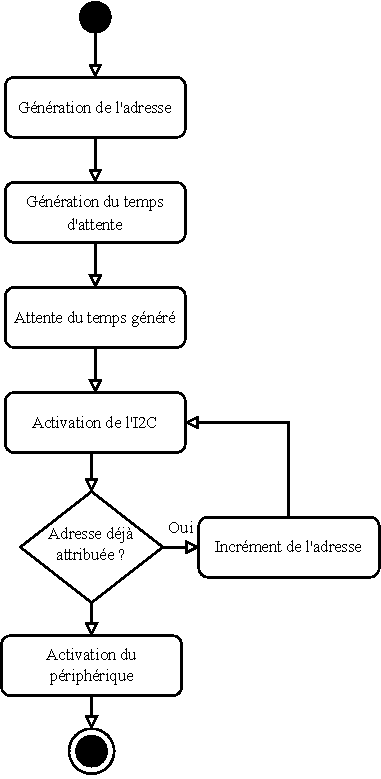
\includegraphics[scale=1.3]{./assets/figures/gen_addr.pdf}
    \caption{Algorithme de génération d'adresse \gls{i2c}}
\end{figure}

\section{CI/CD}

L'intégration continue (CI) et le déploiement continu (CD) sont deux pratiques utilisées dans le développement de logiciels pour améliorer la qualité, la rapidité et l'efficacité du processus de développement.

\subsection{Définitions}

L'intégration continue consiste à fusionner régulièrement le code développé par les différents membres d'une équipe dans un référentiel central.
Cela permet de détecter rapidement les éventuels problèmes d'incompatibilité ou d'erreur de code, car chaque modification est automatiquement testée et intégrée au code existant.
Les développeurs reçoivent ainsi rapidement des informations sur la validité de leurs modifications, ce qui permet de corriger les erreurs plus tôt dans le processus de développement.

Le déploiement continu, quant à lui, va plus loin en automatisant la phase de déploiement du logiciel.
Une fois que le code a été intégré et testé avec succès, le processus de déploiement se déclenche automatiquement, permettant ainsi la mise à disposition rapide du logiciel aux utilisateurs finaux.
Cela peut inclure le déploiement sur des serveurs de production, la mise à jour des applications ou même la publication sur des plateformes d'applications.

En combinant l'intégration continue et le déploiement continu, les équipes de développement peuvent assurer une livraison plus fréquente et plus fiable des fonctionnalités du logiciel.
Les tests automatisés et l'automatisation du déploiement réduisent les risques d'erreurs, de conflits de code et de problèmes de déploiement, tout en accélérant le cycle de développement global.
Cela permet aux équipes de fournir plus rapidement de nouvelles fonctionnalités et de répondre aux besoins changeants des utilisateurs de manière plus efficace.

\subsection{Objectifs}

Au sein du projet, l'utilisation de l'intégration continue et du déploiement continu est considérée comme une approche pertinente.
L'objectif est d'automatiser la mise à jour du micrologiciel embarqué des périphériques concernés au sein de l'écosystème en cas de modifications apportées à la base de code.
Lorsqu'une mise à jour est effectuée, le système effectue une vérification de la faisabilité de la construction du micrologiciel, puis procède automatiquement au déploiement sur les périphériques.

\subsection{Fonctionnement}

L'utilisation de GitHub pour mettre en place le système de CI/CD est pertinente en raison de sa vaste communauté et des nombreux paquets disponibles pour automatiser diverses tâches.
Le processus comporte deux étapes principales.

Dans un premier temps, l'objectif est de compiler le code afin de générer le fichier binaire du micrologiciel, qui pourra ensuite être téléversé sur un microcontrôleur.

Dans un deuxième temps, il est souhaitable de téléverser le micrologiciel sur les microcontrôleurs concernés, si cela est possible.
Cette étape nécessite une attention particulière, car le maître \gls{i2c} doit être connecté à Internet.
Si tel est le cas, il peut recevoir une notification indiquant la disponibilité d'une nouvelle version du micrologiciel et procéder à sa mise à jour directement sur les microcontrôleurs. Dans le cas où le maître \gls{i2c} ne dispose pas d'une connexion Internet, la mise à jour sera effectuée dès que le maître \gls{i2c} sera allumé et connecté à Internet.

En résumé, le système présenté offre la possibilité de mettre à jour les composants du bus \gls{i2c} de manière automatique en modifiant le code sur Github à partir de n'importe quel ordinateur.
Cette approche présente un avantage significatif en termes de flexibilité, évitant ainsi les contraintes liées à une mise à jour traditionnelle qui exige l'utilisation d'un câble de reprogrammation pour chaque périphérique.

\section{Gestion des erreurs}

La gestion des erreurs n'étant pas prise en charge de manière native sur un bus \gls{i2c}, il est pertinent de mettre en place un système de secours pour redémarrer les périphériques en cas de problèmes.
Dans un premier temps, il est nécessaire de détecter les erreurs.
Cette tâche peut être complexe à première vue, car les erreurs doivent être détectées depuis les périphériques esclaves du bus, étant donné que c'est l'élément contrôlé de manière totale.

Dans un deuxième temps, il est requis de trouver une solution pour résoudre le problème.
La solution la plus simple consiste à redémarrer le microcontrôleur.
Cela garantit que si le maître \gls{i2c} bloque la communication sur le périphérique, le redémarrage mettra fin à cet échange et réglera le problème.

Afin d'explorer les différentes solutions possibles pour détecter les erreurs de manière efficace, cette section se concentrera sur cette problématique.

\subsection{Passage en mode maître}

Une solution envisagée pour détecter les erreurs sur le bus \gls{i2c} consiste à transformer périodiquement les esclaves \gls{i2c} en maîtres pour analyser le bus.
Cela permettrait de détecter facilement les erreurs sur le bus.
Cependant, cette approche présente un désavantage important : lorsque le périphérique est en mode maître, il n'est plus disponible en tant qu'esclave pour répondre à ses tâches habituelles.

Ce désavantage rend cette solution non viable, car il est inacceptable de rendre le système inopérant pour détecter les erreurs du bus.

\subsection{Analyse des signaux}

L'analyse des signaux est une solution qui consiste à déterminer ce qui est acceptable sur les signaux de l'\gls{i2c} soit SDA et SCL. Une fois le comportement déterminé, il est possible de déterminer un comportement qui pose problème. En tant qu'esclave du bus \gls{i2c}, il est possible d'analyser les signaux du bus \gls{i2c} sans mettre en péril les communications \gls{i2c} courantes.
\chapter{Implémentation}
Dans ce chapitre, l'objectif est de fournir une explication détaillée de l'implémentation de chaque composant du projet, en mettant en évidence les choix techniques qui ont été faits.
Cela permet de donner une vue d'ensemble du projet et d'expliquer les raisons pour lesquelles chaque partie a été mise en place de cette manière spécifique.

\section{Matériel}

Pour la mise en place et les tests de ce projet, plusieurs composants matériels sont nécessaires.

Tout d'abord, il est nécessaire d'avoir une unité qui agit comme le maître I2C.
Dans ce cas, un Raspberry Pi modèle 3 a été utilisé.
Il est possible d'utiliser une autre carte, à condition qu'elle permette d'installer un système d'exploitation capable d'exécuter du code Python.
De plus, il est important d'avoir une connexion I2C disponible.
Dans ce projet, le Raspberry Pi est équipé de Raspbian.

Ensuite, des cartes de développement sont nécessaires pour tester rapidement le code.
STMicroelectronics fournit une gamme de cartes Nucleo équipées de microcontrôleurs STM32.
La carte NUCLEO-G071RB possède un microcontrôleur STM32 très similaire à celui sélectionné pour ce projet, ce qui la rend idéale pour les tests.
De plus, elle est équipée d'un connecteur ST-Link qui permet de programmer le microcontrôleur directement depuis un ordinateur via USB.
Étant donné que c'est une carte de développement, il est facile de connecter des éléments au microcontrôleur via les GPIO.

\begin{figure}[H]
    \centering
    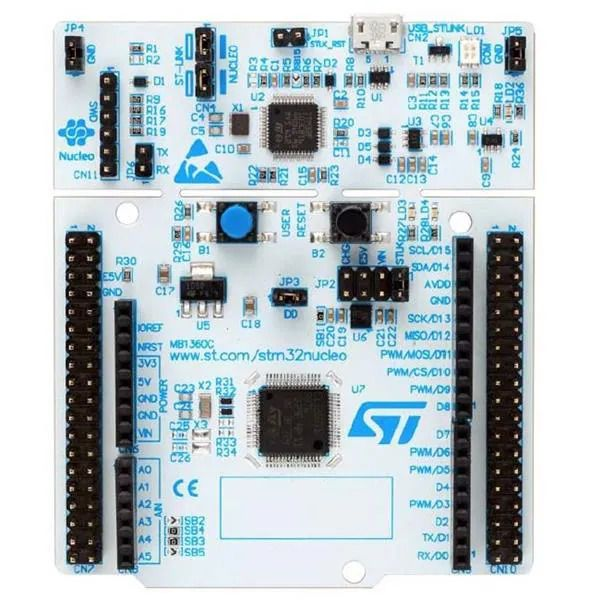
\includegraphics[scale=0.2]{./assets/figures/nucleo.jpg}
    \caption{\cite{nucleo} Carte Nucleo}
\end{figure}

En cas de problème sur le bus I2C, un analyseur logique peut être utile pour observer ce qui se passe.
Dans ce projet, un Saleae Logic 8 a été utilisé.
Cet analyseur logique est pratique pour diagnostiquer les problèmes de communication.
Il permet souvent d'identifier quel composant pose problème et de cibler plus rapidement la source du dysfonctionnement.

En résumé, avec un Raspberry Pi, plusieurs cartes Nucleo servant d'esclaves I2C, il est possible de tester l'intégralité du projet.

\section{Logiciels}

Dans cette section, les différents logiciels utilisés dans ce projet seront décrits, en mettant en évidence leur utilité, leur fonctionnement, ainsi que leurs avantages et inconvénients.

\subsection{PlatformIO}

PlatformIO est un environnement de développement intégré (IDE) qui se présente sous la forme d'une extension pour Visual Studio Code.
Il offre la gestion de plus de cinquante plateformes, plus de vingt \textit{\gls{framework}}s et plus de treize mille bibliothèques.
Cet outil est particulièrement pratique pour explorer rapidement et facilement les différents \textit{\gls{framework}}s compatibles avec les cartes de développement.
Dans le cadre de ce projet, il a été utilisé pour explorer les différentes options de \textit{\gls{framework}}s.
Son principal avantage réside dans sa polyvalence, car il permet de gérer un large éventail de plateformes et de \textit{\gls{framework}}s.
Cependant, sa polyvalence peut également être considérée comme un inconvénient, car il n'est pas optimisé pour un \textit{\gls{framework}} spécifique.

\subsection{Mbed Studio}

Mbed Studio est un environnement de développement intégré (IDE) développé par Arm pour les microcontrôleurs.
Il est basé sur Visual Studio Code et est spécifiquement optimisé pour les microcontrôleurs.
Mbed Studio permet de gérer les cartes de développement de STMicroelectronics, mais il est également possible d'ajouter des cartes de développement d'autres fabricants.
L'un des avantages majeurs de Mbed Studio est sa facilité de débogage, car il permet de déboguer le code directement sur une carte de développement.
Cette fonctionnalité s'avère très pratique lorsqu'on rencontre des comportements indéterminés dans le code.

Dans ce projet, Mbed Studio a été utilisé une fois que le \textit{\gls{framework}} Mbed a été choisi.
Il a permis de gagner du temps en facilitant le processus de débogage.

\section{Mise à jour du micrologiciel}

Dans cette section, le processus de mise à jour du micrologiciel via le bus I2C sera expliqué en détail.
Les deux méthodes possibles pour effectuer la mise à jour seront présentées, en mettant en avant leurs avantages et leurs inconvénients respectifs.

Il existe deux approches pour la mise à jour du micrologiciel via le bus I2C.
La première méthode consiste à télécharger le nouveau micrologiciel à partir de l'application exécutée par le microcontrôleur.
Cela nécessite que le microcontrôleur dispose d'une quantité suffisante de mémoire pour stocker les deux micrologiciels.
Ainsi au redémarrage, le chargeur de démarrage remplace l'ancien micrologiciel par le nouveau.
Cependant, cette méthode nécessite une capacité de mémoire plus importante, car elle nécessite le stockage des deux micrologiciels.

La deuxième méthode consiste à aller dans le chargeur de démarrage pour effectuer la mise à jour.
Dans ce mode, le microcontrôleur est capable de recevoir le nouveau micrologiciel et de le programmer en mémoire.
Cette approche évite le besoin de stocker les deux micrologiciels simultanément, mais elle nécessite que le chargeur de démarrage soit équipé de la fonctionnalité de mise à jour complète.

Chaque méthode présente ses avantages et ses inconvénients.
La première méthode permet une mise à jour plus facile et rapide à partir de l'application, mais elle nécessite une mémoire plus importante.
La deuxième méthode nécessite une fonctionnalité de mise à jour dans le bootloader, mais elle peut être utilisée même si la mémoire disponible est limitée.

\subsection{Envoi du micrologiciel}

L'envoi du micrologiciel se fait par morceaux étant donné que la mémoire vive du microcontrôleur ne peut pas contenir le micrologiciel complet en même temps, en raison de l'utilisation de la mémoire vive par l'application en cours d'exécution.
Les données du micrologiciel sont stockées dans un tampon déclaré dans le code, qui lui est stocké dans la mémoire vive.

La mémoire vive du microcontrôleur choisi a une capacité de 36 kilo-octets.
La taille d'un micrologiciel avec Mbed, incluant une simple réponse I2C, est d'environ 30 kilo-octets.
L'ajout de fonctionnalités supplémentaires augmentera la taille du micrologiciel.

La taille des morceaux a été fixée à 1024 octets. Cette valeur a été sélectionnée pour sa facilité de représentation en termes du nombre de morceaux qui seront envoyés pour le micrologiciel.
De plus, cette taille s'adapte parfaitement à la mémoire vive, même en cas d'utilisation intensive.
Il s'agit d'une taille pertinente qui permet d'optimiser le temps d'envoi en termes du nombre de morceaux, tout en minimisant le temps d'écriture sur la mémoire flash entre deux communications I2C.

\subsection{Detection d'un micrologiciel valide}

Il est impératif que le chargeur de démarrage détecte la présence d'un micrologiciel.
Pour une détection rapide, l'application Mbed comporte une en-tête pré-définie contenant des informations spécifiques.
La première information est un nombre magique, identique à chaque fois et préalablement connu par le chargeur de démarrage.
Ainsi, ce dernier peut simplement vérifier si la première donnée de l'en-tête correspond effectivement au nombre magique prévu.

Ensuite, il est nécessaire de garantir la validité du micrologiciel.
Pour cela, Mbed permet d'ajouter un code de \gls{crc} dans l'en-tête de l'application, qui est automatiquement calculé lors de la génération de l'application.
Le chargeur de démarrage peut alors calculer le \gls{crc} de l'application et le comparer à celui de l'en-tête.
Si les deux \gls{crc} correspondent, cela signifie que le micrologiciel est valide.

Le \gls{crc} est un mécanisme utilisé pour détecter les erreurs de transmission de données.
Il consiste à générer un code de contrôle en effectuant des calculs mathématiques sur les données à transmettre.
Comme il s'agit d'un calcul, il peut être recalculé lors de la réception.

Grâce à ces vérifications, il est assuré que le micrologiciel est valide et que le démarrage de l'application est possible.

\subsection{Mise à jour par l'application}

Dans cette solution, l'utilisateur envoie les données du nouveau micrologiciel directement à l'application s'exécutant sur le microcontrôleur.
L'application reçoit un morceau de données via le bus I2C et l'écrit dans une zone mémoire réservée au nouveau micrologiciel dans la mémoire flash.
Une fois toutes les données du micrologiciel reçues, le microcontrôleur redémarre.
Le chargeur de démarrage doit détecter la présence d'un nouveau micrologiciel dans la zone mémoire réservée.
S'il détecte un micrologiciel valide, il peut le copier à la place de l'ancien micrologiciel.
Une vérification est ensuite effectuée pour s'assurer que la copie s'est déroulée correctement.

Pour implémenter cette solution, lors de la communication I2C entre le maître et le microcontrôleur, un numéro de registre doit être spécifié.
Ce numéro indique à l'application qu'il s'agit d'un message de mise à jour du micrologiciel.
Étant donné que le nouveau micrologiciel est divisé en morceaux, il est nécessaire d'envoyer à la fois le numéro du morceau et le nombre total de morceaux.
Ainsi, l'application peut placer correctement les données dans la mémoire flash.

\begin{figure}[H]
    \centering
    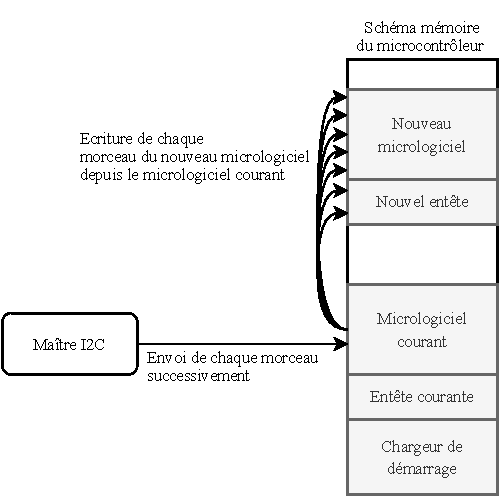
\includegraphics[scale=1.3]{./assets/figures/firmware_update.pdf}
    \caption{Schéma de mise à jour par l'application}
\end{figure}

\subsection{Mise à jour par le chargeur de démarrage}

Dans cette solution, la responsabilité de la mise à jour du micrologiciel repose sur le chargeur de démarrage.
Lorsque l'application du microcontrôleur reçoit l'indication de mettre à jour le micrologiciel via I2C, elle redémarre pour permettre au chargeur de démarrage de prendre le relais.
Cependant, il est nécessaire d'informer le chargeur de démarrage d'attendre une mise à jour et de ne pas démarrer sur le micrologiciel actuel.
Pour ce faire, le chargeur de démarrage s'arrête et attend une mise à jour dans certaines conditions :

\begin{itemize}
    \item L'application doit être mise à jour.
    \item L'application ne présente pas le bon nombre magique.
    \item L'application ne présente pas le bon \gls{crc}.
\end{itemize}

L'application peut se qualifiée de "sujette à mise à jour".
En conséquence, le chargeur de démarrage peut être programmé pour attendre une mise à jour tant que le nombre magique et le \gls{crc} sont corrects.

Une fois que le chargeur de démarrage sait qu'il doit attendre une mise à jour, il reste en attente de la mise à jour via le bus I2C.
Une fois que le nouveau micrologiciel est reçu et vérifié, le chargeur de démarrage démarre avec le nouveau micrologiciel.
Le système de mise à jour a été influencé par la référence \cite{reindl2020software}.

\begin{figure}[H]
    \centering
    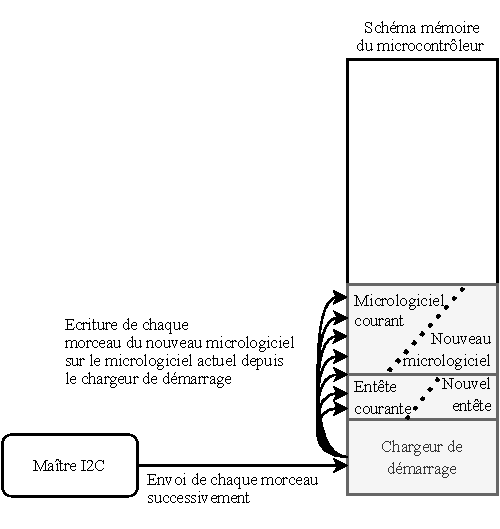
\includegraphics[scale=1.3]{./assets/figures/bootloader_update.pdf}
    \caption{Schéma de mise à jour par le chargeur de démarrage}
\end{figure}

L'avantage de cette solution réside dans la possibilité de mettre à jour le micrologiciel même si l'application est corrompue ou si elle ne gère pas correctement le redémarrage vers le chargeur de démarrage.
Toutefois, la gestion du bus I2C peut être effectuée par le chargeur de démarrage ou par le micrologiciel.

\subsection{Stockage des métadonnées}

Il est nécessaire de permettre la mise à jour du micrologiciel tout en préservant les métadonnées associées.
Cela implique de conserver le nom, le groupe et le type de capteur.
La perte de ces informations à chaque mise à jour serait incohérente.
Par conséquent, il est essentiel de stocker ces données en dehors de la zone mémoire du micrologiciel.
Cependant, elles ne doivent pas faire partie du chargeur de démarrage commun à tous les périphériques.

La solution consiste à réserver une zone mémoire entre le chargeur de démarrage et le micrologiciel.
Ainsi, le micrologiciel peut être mis à jour tout en conservant ses métadonnées, sans les inscrire dans le chargeur de démarrage.

Pour mettre cela en \oe{}uvre, il est nécessaire de réserver plus d'espace pour le chargeur de démarrage.
Cela augmentera sa taille, mais n'utilisera pas la fin de la zone mémoire réservée. Pour faciliter l'effacement et l'écriture des données, il est préférable de choisir une taille de données correspondant à celle d'un secteur pour le microcontrôleur.
Cela permettra aux fonctions d'écriture et d'effacement de mbed de fonctionner de manière optimale.
En effet, la gestion de la mémoire flash se fait par secteurs.
Par conséquent, il est préférable d'adapter la taille réservée pour les métadonnées à la taille d'un secteur et de l'aligner correctement.

Grâce à cette méthode, il est possible de stocker des données liées à une carte qui peuvent être modifiées à la fois par le chargeur de démarrage et par le micrologiciel, tout en maintenant leur intégrité même après une mise à jour complète du micrologiciel.

\begin{figure}[H]
    \centering
    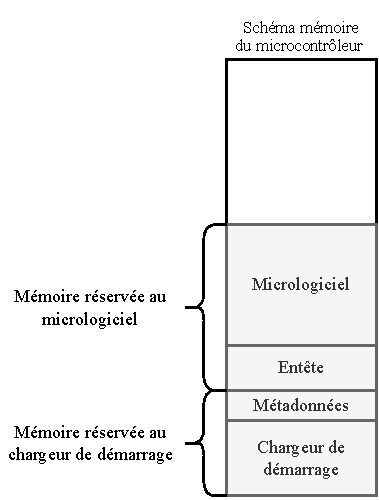
\includegraphics[scale=1.3]{./assets/figures/metadata.pdf}
    \caption{Schéma de la répartition mémoire du microcontrôleur avec les métadonnées}
\end{figure}

\section{Interface POSIX}

Dans cette section, la mise en \oe{}uvre de l'interface POSIX sera détaillée. L'explication des raisons pour lesquelles l'interface a été mise en \oe{}uvre de cette manière et les choix effectués seront abordés.

\subsection{Environnement}

Dans ce projet, aucun environnement matériel final n'est défini. L'objectif consiste à créer un écosystème sur le bus I2C qui peut être réutilisé par d'autres projets. Par conséquent, une interface doit être développée pour être utilisée avec la plupart des maîtres I2C.

Il existe deux types de maîtres I2C possibles. Un maître équipé d'un système d'exploitation, généralement Linux, et un maître sans système d'exploitation, généralement un microcontrôleur. Il convient toutefois de noter qu'une fonctionnalité importante de l'interface POSIX est le déploiement de nouveaux micrologiciels. Par conséquent, le maître I2C doit être capable de mettre à jour, puis de compiler et finalement d'envoyer le micrologiciel.

\subsection{Choix du langage}

En prenant en compte les deux types de maîtres possibles, il convient de déterminer lequel est plus approprié à mettre en avant.
Étant donné la nécessité de modifier et de compiler le code avant de pouvoir l'envoyer, il est peu pertinent de privilégier le maître basé sur un microcontrôleur avec l'écosystème développé.
Par conséquent, il est plus intéressant de construire une interface fonctionnant sur un système d'exploitation. Les explications d'implémentation détaillées permettront, si nécessaire, de créer une interface adaptée à un environnement plus spécifique.

Plusieurs options sont envisageables en ce qui concerne le langage de programmation.
Il est possible d'opter pour un langage tel que C ou C++, ou bien de se tourner vers Python.
Étant donné qu'il s'agit davantage de scripts avancés que d'un véritable programme, il est plus intéressant d'utiliser Python.
Il convient parfaitement à la réalisation d'une interface POSIX et bénéficie de bibliothèques facilitant le développement.

\subsection{Fonctionnement}

Dans cette sous-section, l'objectif consiste à expliquer l'implémentation de chaque partie de l'interface POSIX.
Cela permet de comprendre les choix effectués et d'adapter l'interface POSIX en fonction des besoins spécifiques.

\subsubsection{Mise à jour du micrologiciel}

\todo{Fonctionnement de la mise à jour du micrologiciel}

\subsubsection{Analyse du bus}

\todo{Fonctionnement de l'analyse du bus}


\chapter{Démonstrateur}
Dans ce chapitre, l'objectif est d'expliquer les choix effectués pour la réalisation d'un démonstrateur fonctionnel mettant en évidence la partie matérielle de ce projet.
Le démonstrateur se présente sous la forme d'un circuit imprimé intégrant le microcontrôleur sélectionné.

Ce démonstrateur a été conçu en tenant compte de son utilisation potentielle lors des prochaines éditions du concours Eurobot, auquel participe le club de robotique de la \gls{heigvd}.

\section{Fonctionnalités}

L'objectif de ce démonstrateur est de mettre en évidence les fonctionnalités de l'écosystème I2C de ce projet.
Pour cela, un circuit imprimé a été conçu, intégrant le microcontrôleur choisi, un capteur de couleur et une LED.
Ce démonstrateur permet de démontrer toutes les fonctionnalités et peut être utilisé au sein du club de robotique de la \gls{heigvd} lors des prochaines éditions du concours Eurobot.

\section{Tension electrique}

La tension électrique d'un périphérique sur le bus I2C n'est pas fixée selon une norme précise.
Cependant, il est courant d'utiliser deux tensions électriques différentes : 3,3V et 5V.
Dans le cadre de ce projet, il est préférable de choisir une tension compatible avec le microcontrôleur sélectionné.
Selon la fiche technique du microcontrôleur, la tension d'alimentation recommandée est de 1,71V à 3,6V.
Il est donc logique d'opter pour une tension de 3,3V pour le bus I2C.
Cela permet de simplifier le circuit en évitant d'avoir plusieurs composants électroniques pour abaisser la tension du bus.

\section{Connecteurs}

Le choix du connecteur est un aspect important à considérer.
Il doit être à la fois compact et solide.
La compacité est essentielle pour minimiser la taille du circuit imprimé, en accord avec l'aspect embarqué du projet.
La solidité du connecteur est primordiale afin de garantir une connexion fiable, même en cas de branchement et débranchement fréquents.

Le connecteur sélectionné doit comporter quatre broches pour l'I2C, comprenant l'alimentation du circuit imprimé (3,3V et GND) ainsi que les broches pour l'I2C (SDA et SCL).

Dans le cadre de ce projet, deux connecteurs ont été analysés.
Le connecteur QWIIC de Sparkfun, largement utilisé pour les périphériques I2C, et le connecteur Micro MaTch de TE Connectivity.

\subsection{QWIIC}

Le connecteur QWIIC proposé par Sparkfun est compact.
En effet, pour un connecteur à quatre broches, la partie s'intégrant au circuit imprimé mesure 2,95 mm de hauteur, 6,25 mm de longueur et 7 mm de largeur.
Cependant, il peut être difficile de l'assembler soi-même sans l'outil approprié.
Il est préférable d'acheter des câbles pré-confectionnés, mais cela limite la possibilité de réaliser des câbles sur mesure sans avoir besoin de connecteurs supplémentaires.

\begin{figure}[H]
    \centering
    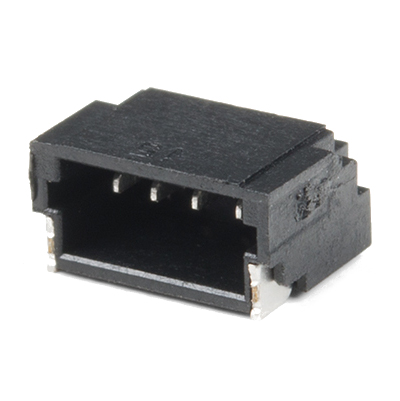
\includegraphics[scale=0.6]{./assets/figures/qwiic.jpg}
    \caption{\cite{qwiic} Connecteur QWIIC}
\end{figure}

En résumé, le connecteur QWIIC est compact mais peut être difficile à assembler sans l'outil approprié.

\subsection{Micro MaTch}

Le connecteur Micro MaTch, fabriqué par la société suisse TE Connectivity, présente l'avantage de pouvoir être assemblé manuellement avec des câbles plats.
En effet, les deux parties du connecteur viennent pincer le câble plat, établissant ainsi la connexion électrique.
La taille du connecteur pour quatre broches sur le circuit imprimé mesure 5,3 mm de hauteur, 6,9 mm de longueur et 9,7 mm de largeur.

\begin{figure}[H]
    \centering
    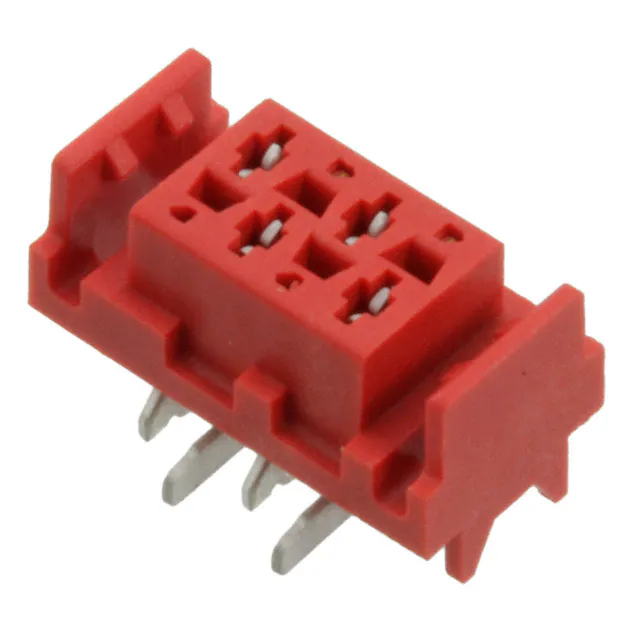
\includegraphics[scale=0.08]{./assets/figures/micromatch.png}
    \caption{\cite{micromatch} Connecteur Micro MaTch}
\end{figure}

En résumé, il est facile d'assembler le connecteur Micro MaTch à un câble plat, mais il n'est pas aussi compact que le connecteur QWIIC.

\subsection{Choix}

Le choix s'est porté sur le connecteur Micro MaTch.
En effet, il est facile à assembler manuellement et offre une compacité satisfaisante.
Bien qu'il soit légèrement moins compact que le connecteur QWIIC, cette différence ne pose pas de problème majeur.
Il est préférable d'avoir un connecteur légèrement plus grand en échange d'une meilleure solidité.
L'avantage principal du connecteur Micro MaTch est la possibilité de l'assembler manuellement sans avoir besoin d'un équipement spécifique.
La référence du connecteur Micro Match choisi est 338069-4.

Cependant, il est important de noter que le connecteur n'est pas un élément essentiel. Il peut être remplacé par un autre connecteur existant pour s'adapter à d'autres projets. Un minimum de 4 broches est nécessaire pour l'alimentation et l'I2C.

\section{Circuit imprimé}

La conception du circuit imprimé a été confiée à l'institut d'automatisation industrielle (IAI) de la \gls{heigvd}, afin de maintenir une conception interne offrant une flexibilité pour les modifications ultérieures.
Cette approche permet également de maintenir une cohérence avec les autres projets de l'institut.
Le logiciel Altium Designer a été utilisé pour concevoir le circuit imprimé, en veillant à ce qu'il soit aussi compact que possible tout en facilitant la soudure.
Le circuit a été commandé chez Eurocircuit, et la soudure des composants a été réalisée par l'institut d'automatisation industrielle.

\section{Débogueur}

Il est possible d'effectuer la mise à jour du nouveau micrologiciel du microcontrôleur via le bus I2C.
Cependant, pour assurer son fonctionnement, il est nécessaire que le chargeur de démarrage préalablement développé dans le projet soit déjà présent.
Ainsi, il est nécessaire d'avoir un moyen d'implanter initialement le chargeur de démarrage sur le microcontrôleur.
À cet effet, il est requis de disposer d'un connecteur sur le circuit imprimé permettant d'accéder aux broches de programmation.
Le système de connecteur Tag Connect a été choisi à cet effet, car il présente uniquement des trous sur le circuit imprimé.
La connexion s'effectue à l'aide d'un câble spécifique.

\begin{figure}[H]
    \centering
    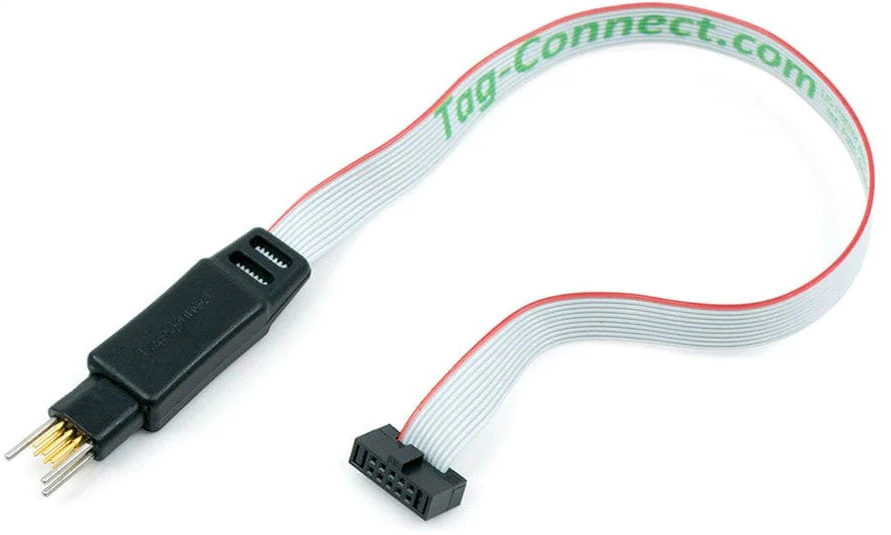
\includegraphics[scale=0.2]{./assets/figures/tag_connect.png}
    \caption{\cite{tag_connect} Câble Tag Connect}
\end{figure}

\begin{figure}[H]
    \centering
    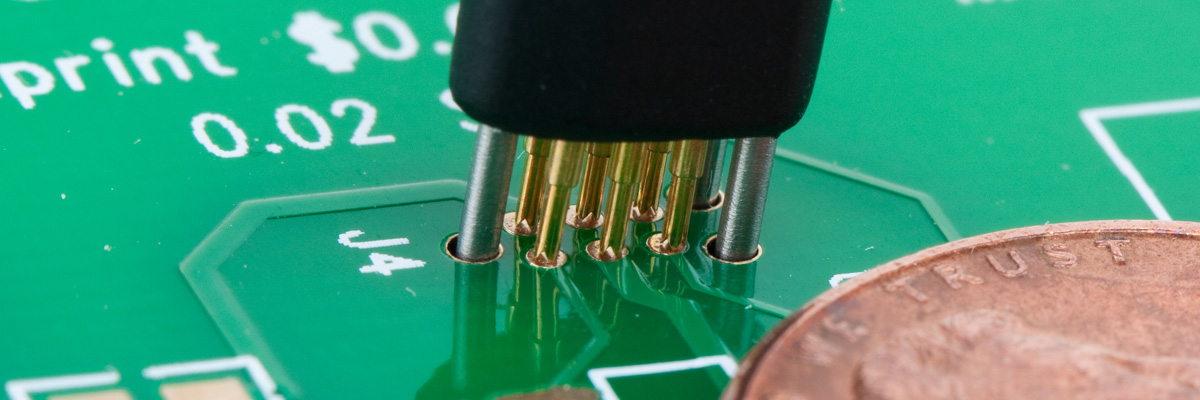
\includegraphics[scale=0.2]{./assets/figures/tag_connect_pcb.jpg}
    \caption{\cite{tag_connect_pcb} Câble Tag Connect connecté au circuit imprimé}
\end{figure}

De plus, un adaptateur est nécessaire pour établir une connexion ST-LINK avec l'ordinateur.
Le ST-LINK est un débogueur et programmateur pour les microcontrôleurs STM8 et STM32, qui assure la liaison entre l'ordinateur et le microcontrôleur.
Grâce à cette configuration, il est possible de programmer le chargeur de démarrage pour la première fois.

\begin{figure}[H]
    \centering
    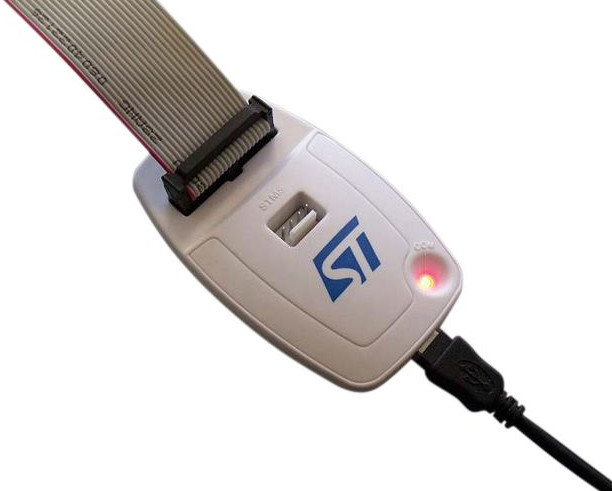
\includegraphics[scale=0.3]{./assets/figures/st_link.jpg}
    \caption{\cite{st_link} Débogueur et programmateur ST-LINK}
\end{figure}

Étant donné que le chargeur de démarrage doit être programmé une seule fois, il serait envisageable de le faire sur une partie fragile du circuit imprimé.
Ainsi, une fois programmé, cette partie fragile pourrait être retirée pour gagner de l'espace sur le circuit imprimé.
Cependant, cette approche n'a pas été utilisée dans le circuit imprimé réalisé, car la programmation du chargeur de démarrage sera réalisée à plusieurs reprises dans le cadre de ce projet.
Par conséquent, il est plus pratique de conserver le connecteur sur le circuit imprimé.

\section{Carte d'extension}

Pour se rapprocher au maximum d'une situation réelle, il est intéressant de mettre en place une carte d'extension pour le Raspberry Pi.
Cette carte d'extension permet d'utiliser le même connecteur que celui choisi sur la carte principale.
Ainsi, il est plus facile de connecter et déconnecter des périphériques plutôt que d'utiliser des câbles Dupont.
Il convient de souligner que cette carte d'extension n'est pas un circuit imprimé sophistiqué, mais simplement une plaque d'expérimentation (veroboard) équipée d'un connecteur et des connexions nécessaires.

\section{Tests}

\todo{Expliquer ce qui a été fait pour tester la carte}



\appendix
\appendixpage
\addappheadtotoc

\chapter{Première annexe}

\let\cleardoublepage\clearpage
\backmatter
% glossaire, biblio et index
\label{glossaire}
\printnoidxglossary
\printbibliography
\label{index}
\printindex



\end{document}
